%!TEX root = ../../super_main.tex

\section{Vision}
\label{sec:vision}

% Vi har ikke nogen udefrakommende kunne, vi vil håndtere dette med et essence vision
This project aims to be innovative and does not have an external customer whom can define and verify requirements. 
\\\\
A methodology that aims to support high value software solutions is Essense \todo{Ref til Essence bog}. Essence mentions having a vision as a great way to start a project. Essence mentions that having different representations of a vision can help elicit objects, events, and qualities to persue. Four different representation types are suggested, namely: Icon, Prototype, Metaphor, Proposition. We have chosen to attempt to represent the existing condition, i.e. the problem area as we understood it at the time, as Icons, Metaphors, and Propositions. We found the prototype representation to costly in terms of development time. 
\\\\
There should be four representations for each type, one for each direction of two, for the project, fundamental questions   should include    must represent solutions


\subsection{Icon Representation}


\subsection{Metaphor Representation}


\subsection{Proposition Representation}


\begin{figure}[!htbp]
    \centering
    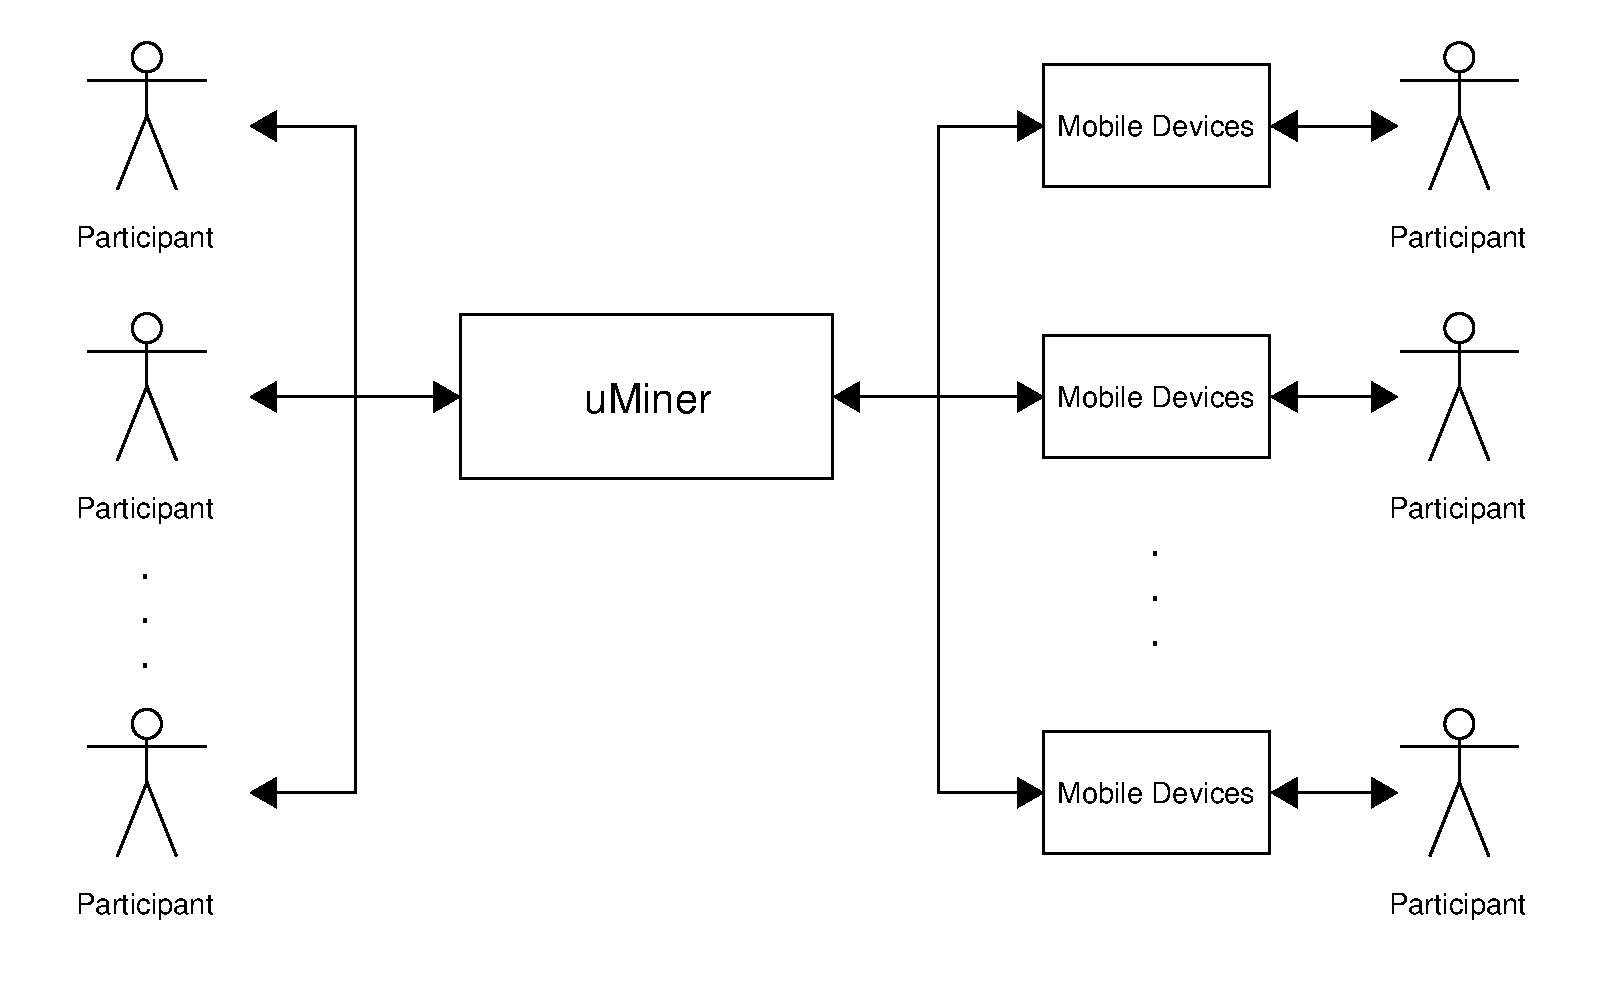
\includegraphics[width=\textwidth]{unsorted/system_vision}
    \caption{The system vision.}
    \label{fig:system_vision}
\end{figure}
\FloatBarrier
